

\tikzset{every picture/.style={line width=0.75pt}} %set default line width to 0.75pt        

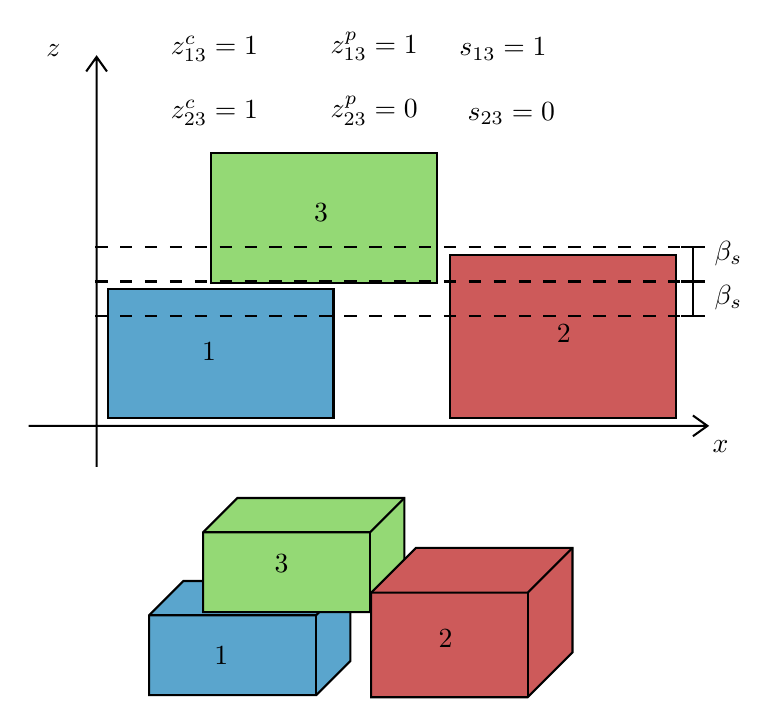
\begin{tikzpicture}[x=0.75pt,y=0.75pt,yscale=-1,xscale=1]
%uncomment if require: \path (0,438); %set diagram left start at 0, and has height of 438

%Shape: Axis 2D [id:dp1232896109350261] 
\draw  (168,199.75) -- (495,199.75)(200.7,22) -- (200.7,219.5) (488,194.75) -- (495,199.75) -- (488,204.75) (195.7,29) -- (200.7,22) -- (205.7,29)  ;
%Shape: Cube [id:dp2910169191165868] 
\draw  [fill={rgb, 255:red, 90; green, 165; blue, 205 }  ,fill opacity=1 ] (226,291) -- (242.5,274.5) -- (323,274.5) -- (323,313) -- (306.5,329.5) -- (226,329.5) -- cycle ; \draw   (323,274.5) -- (306.5,291) -- (226,291) ; \draw   (306.5,291) -- (306.5,329.5) ;
%Shape: Cube [id:dp8785627882196329] 
\draw  [fill={rgb, 255:red, 148; green, 217; blue, 117 }  ,fill opacity=1 ] (252,251) -- (268.5,234.5) -- (349,234.5) -- (349,273) -- (332.5,289.5) -- (252,289.5) -- cycle ; \draw   (349,234.5) -- (332.5,251) -- (252,251) ; \draw   (332.5,251) -- (332.5,289.5) ;
%Shape: Cube [id:dp9708534720424996] 
\draw  [fill={rgb, 255:red, 205; green, 90; blue, 90 }  ,fill opacity=1 ] (333,280.1) -- (354.6,258.5) -- (430,258.5) -- (430,308.9) -- (408.4,330.5) -- (333,330.5) -- cycle ; \draw   (430,258.5) -- (408.4,280.1) -- (333,280.1) ; \draw   (408.4,280.1) -- (408.4,330.5) ;
%Shape: Rectangle [id:dp1912318137049227] 
\draw  [fill={rgb, 255:red, 90; green, 165; blue, 205 }  ,fill opacity=1 ] (206,133.8) -- (314.84,133.8) -- (314.84,196) -- (206,196) -- cycle ;
%Shape: Rectangle [id:dp15878814114025752] 
\draw  [fill={rgb, 255:red, 148; green, 217; blue, 117 }  ,fill opacity=1 ] (255.76,68.5) -- (364.6,68.5) -- (364.6,130.7) -- (255.76,130.7) -- cycle ;
%Shape: Rectangle [id:dp45643376129890645] 
\draw  [fill={rgb, 255:red, 205; green, 90; blue, 90 }  ,fill opacity=1 ] (370.82,117.48) -- (479.66,117.48) -- (479.66,196) -- (370.82,196) -- cycle ;
%Straight Lines [id:da2605780157567503] 
\draw    (488,147) -- (488,130.5) ;
\draw [shift={(488,130.5)}, rotate = 90] [color={rgb, 255:red, 0; green, 0; blue, 0 }  ][line width=0.75]    (0,5.59) -- (0,-5.59)   ;
\draw [shift={(488,147)}, rotate = 90] [color={rgb, 255:red, 0; green, 0; blue, 0 }  ][line width=0.75]    (0,5.59) -- (0,-5.59)   ;
%Straight Lines [id:da24768955122380476] 
\draw  [dash pattern={on 4.5pt off 4.5pt}]  (200,147) -- (488,147) ;
%Straight Lines [id:da896443398249126] 
\draw  [dash pattern={on 4.5pt off 4.5pt}]  (200,130.5) -- (488,130.5) ;
%Straight Lines [id:da13886804211804216] 
\draw    (488,130) -- (488,113.5) ;
\draw [shift={(488,113.5)}, rotate = 90] [color={rgb, 255:red, 0; green, 0; blue, 0 }  ][line width=0.75]    (0,5.59) -- (0,-5.59)   ;
\draw [shift={(488,130)}, rotate = 90] [color={rgb, 255:red, 0; green, 0; blue, 0 }  ][line width=0.75]    (0,5.59) -- (0,-5.59)   ;
%Straight Lines [id:da5108447923150587] 
\draw  [dash pattern={on 4.5pt off 4.5pt}]  (200,130) -- (488,130) ;
%Straight Lines [id:da8065446730531389] 
\draw  [dash pattern={on 4.5pt off 4.5pt}]  (200,113.5) -- (488,113.5) ;

% Text Node
\draw (496,205.4) node [anchor=north west][inner sep=0.75pt]    {$x$};
% Text Node
\draw (175,14.4) node [anchor=north west][inner sep=0.75pt]    {$z$};
% Text Node
\draw (497,130.4) node [anchor=north west][inner sep=0.75pt]    {$\beta _{s}$};
% Text Node
\draw (250,158.4) node [anchor=north west][inner sep=0.75pt]    {$1$};
% Text Node
\draw (421,149.4) node [anchor=north west][inner sep=0.75pt]    {$2$};
% Text Node
\draw (304,91.4) node [anchor=north west][inner sep=0.75pt]    {$3$};
% Text Node
\draw (235,10.4) node [anchor=north west][inner sep=0.75pt]    {$z_{13}^{c} =1$};
% Text Node
\draw (235,41.4) node [anchor=north west][inner sep=0.75pt]    {$z_{23}^{c} =1$};
% Text Node
\draw (312,8.4) node [anchor=north west][inner sep=0.75pt]    {$z_{13}^{p} =1$};
% Text Node
\draw (312,39.4) node [anchor=north west][inner sep=0.75pt]    {$z_{23}^{p} =0$};
% Text Node
\draw (374,11.4) node [anchor=north west][inner sep=0.75pt]    {$s_{13} =1$};
% Text Node
\draw (378,42.4) node [anchor=north west][inner sep=0.75pt]    {$s_{23} =0$};
% Text Node
\draw (256,304.4) node [anchor=north west][inner sep=0.75pt]    {$1$};
% Text Node
\draw (285,260.4) node [anchor=north west][inner sep=0.75pt]    {$3$};
% Text Node
\draw (364,296.4) node [anchor=north west][inner sep=0.75pt]    {$2$};
% Text Node
\draw (497,109.4) node [anchor=north west][inner sep=0.75pt]    {$\beta _{s}$};


\end{tikzpicture}
